\documentclass{article}

% options are:
% - abs: use absolute positioning for the picture
% - percent: use percent positioning for the picture (percent of longer dimension)
% - permil: ten times percent
\usepackage[abs]{overpic}
\usepackage{tikz}
\usepackage{xcolor}
\usepackage[margin=1in]{geometry}

\usetikzlibrary{calc}

% A convenience command to overlay a figure using Tikz
%
% Two versions:
% - \annotatedFigure[]{}{} uses tikz
% - \overlayFigure[]{}{} uses overpic
%
% @param 1: optional arguments to give to \includegraphics (in the square
%           brackets)
% @param 2: content to put in the lower-left corner of the image (e.g., {(a)})
% @param 3: image file path (to give to \includegraphics in curly braces)
%
\newcommand{\annotatedFigure}[3][]{%
  \begin{tikzpicture}[above right, inner sep=0, outer sep=0]
    \node (image) at (0, 0) { \includegraphics[#1]{#3} };
    \node (label) at (1mm, 1mm) {#2};
  \end{tikzpicture}%
}
\newcommand{\overlayFigure}[3][]{%
  \begin{overpic}[
        abs,
        unit=1mm,
        %grid,    % TODO: remove
        %tics=10, % TODO: remove
        #1,
        ]{#3}
    \put(1,2){#2}
  \end{overpic}%
}

\begin{document}

\def\imwidth{0.45\columnwidth}

\begin{figure}
  \centering
  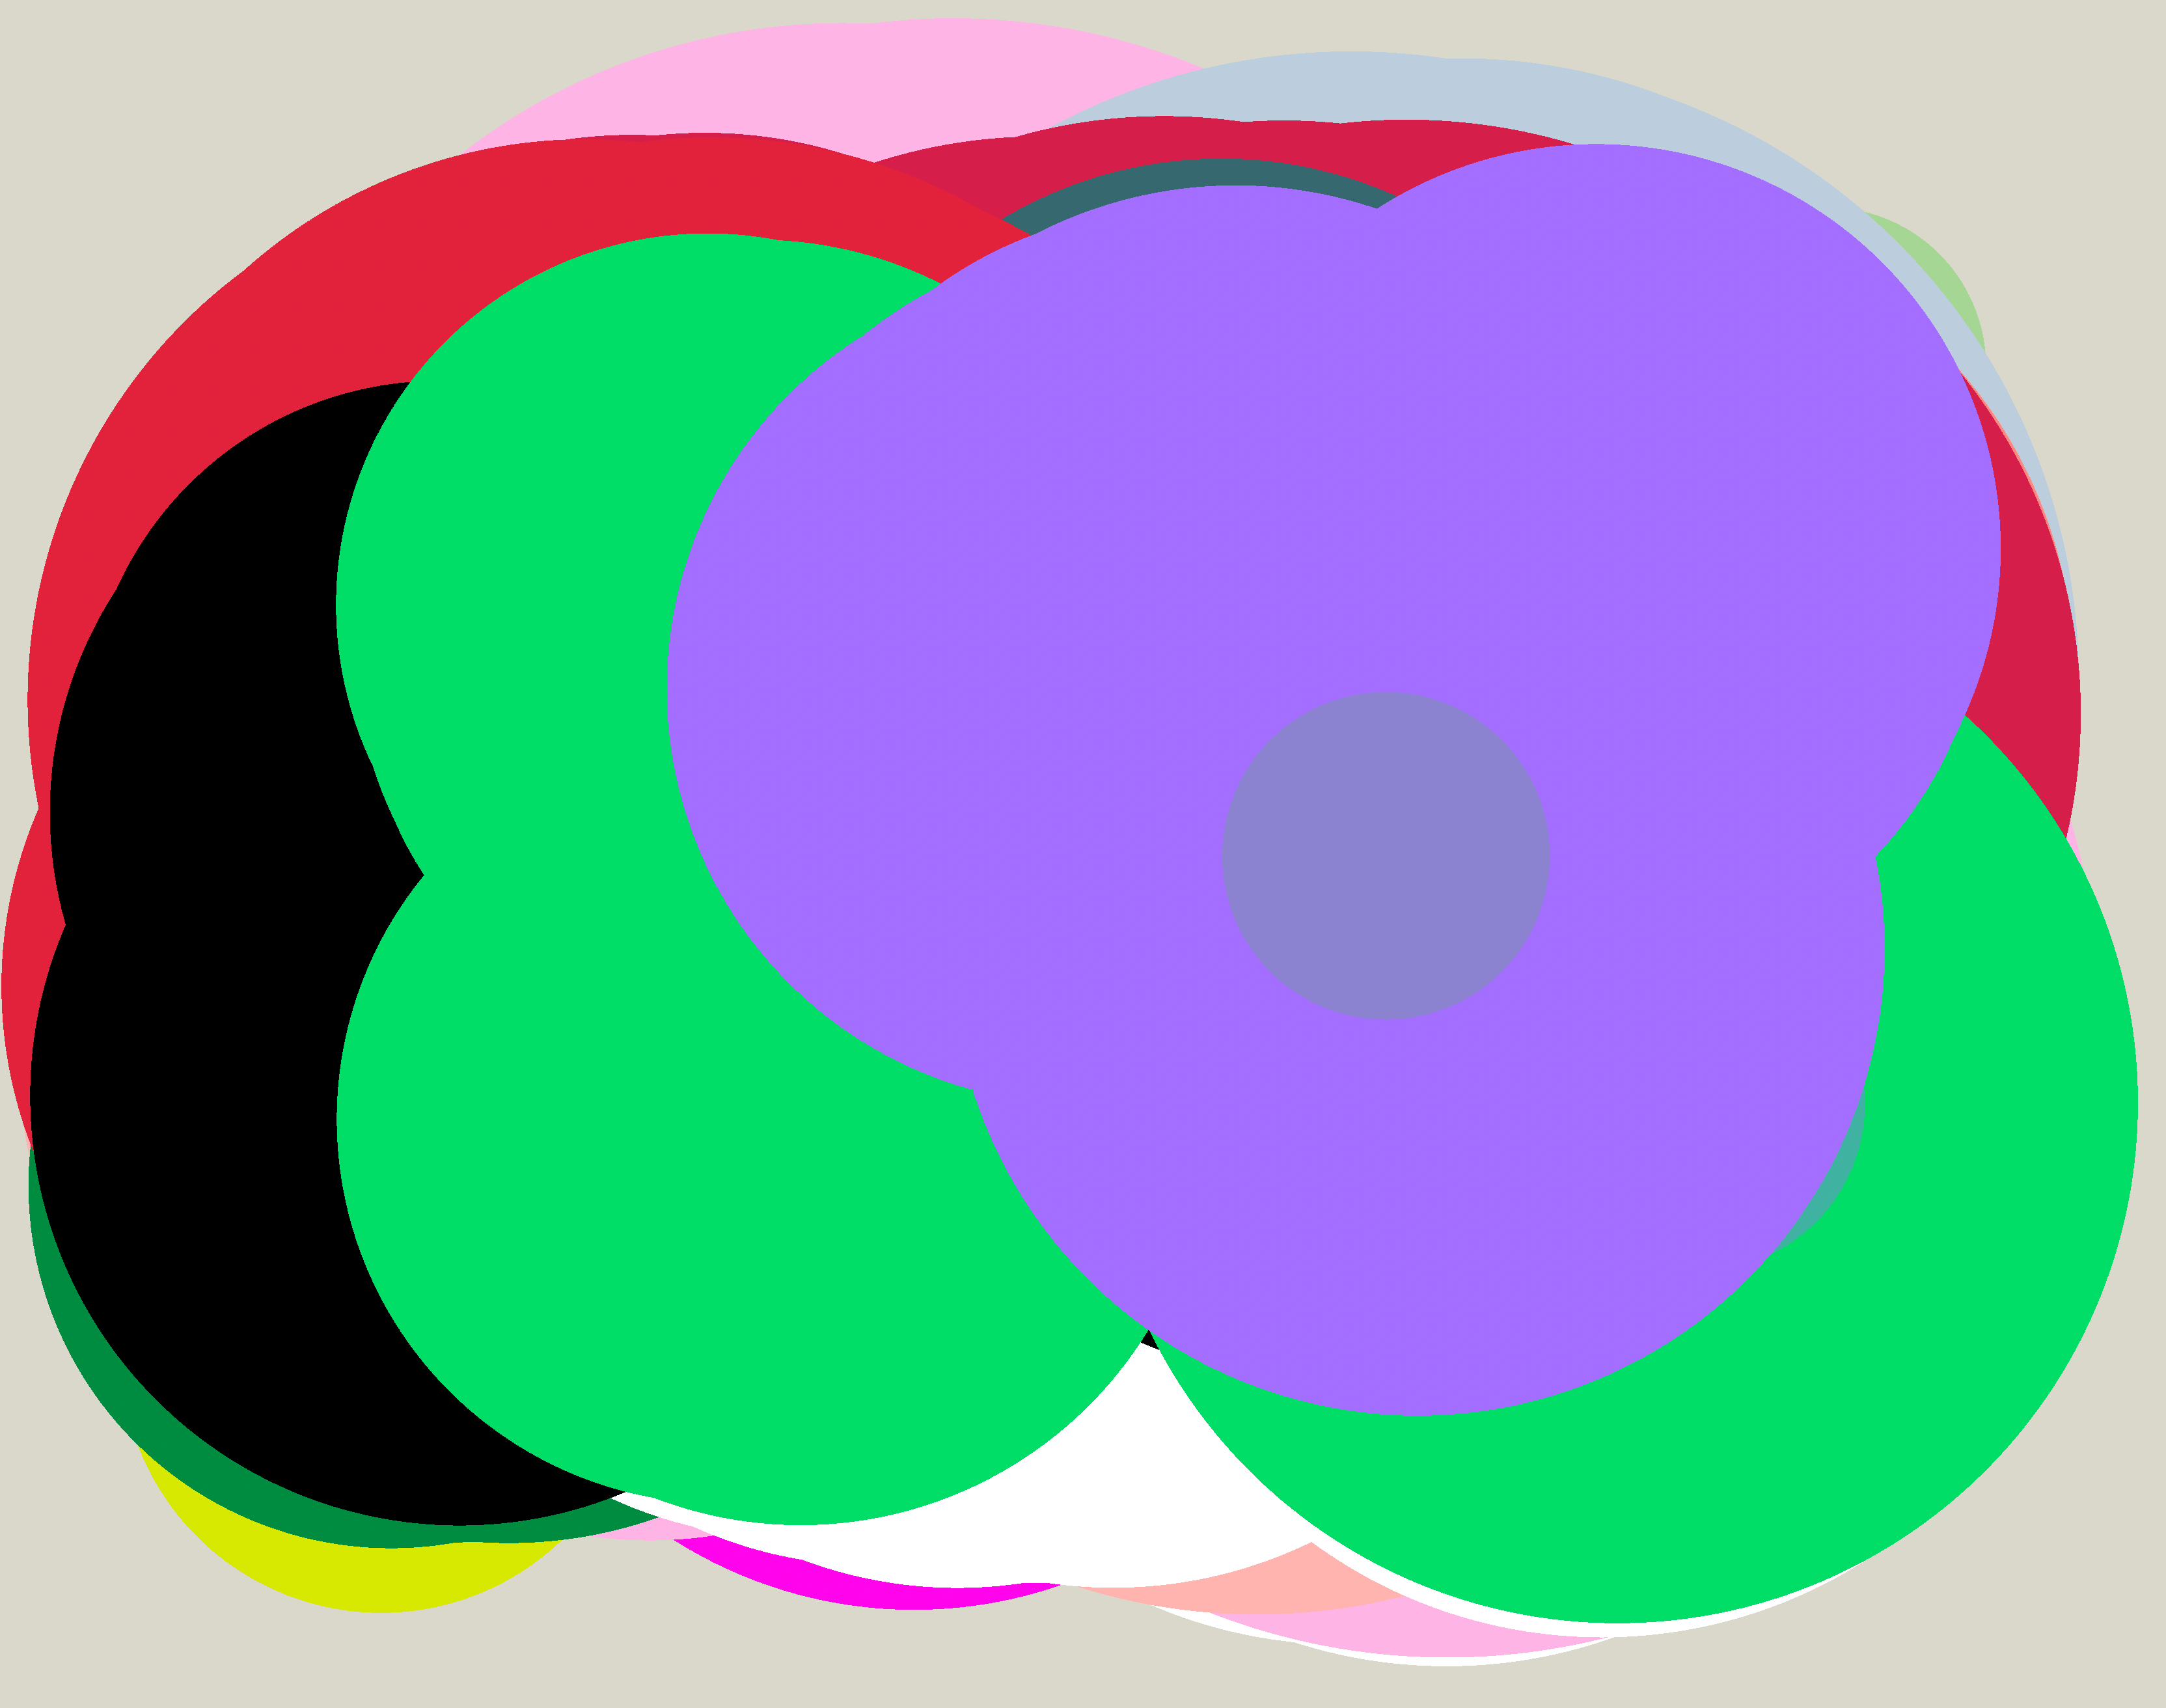
\includegraphics[width=\imwidth]{jack-circles.png}%
  \hfill%
  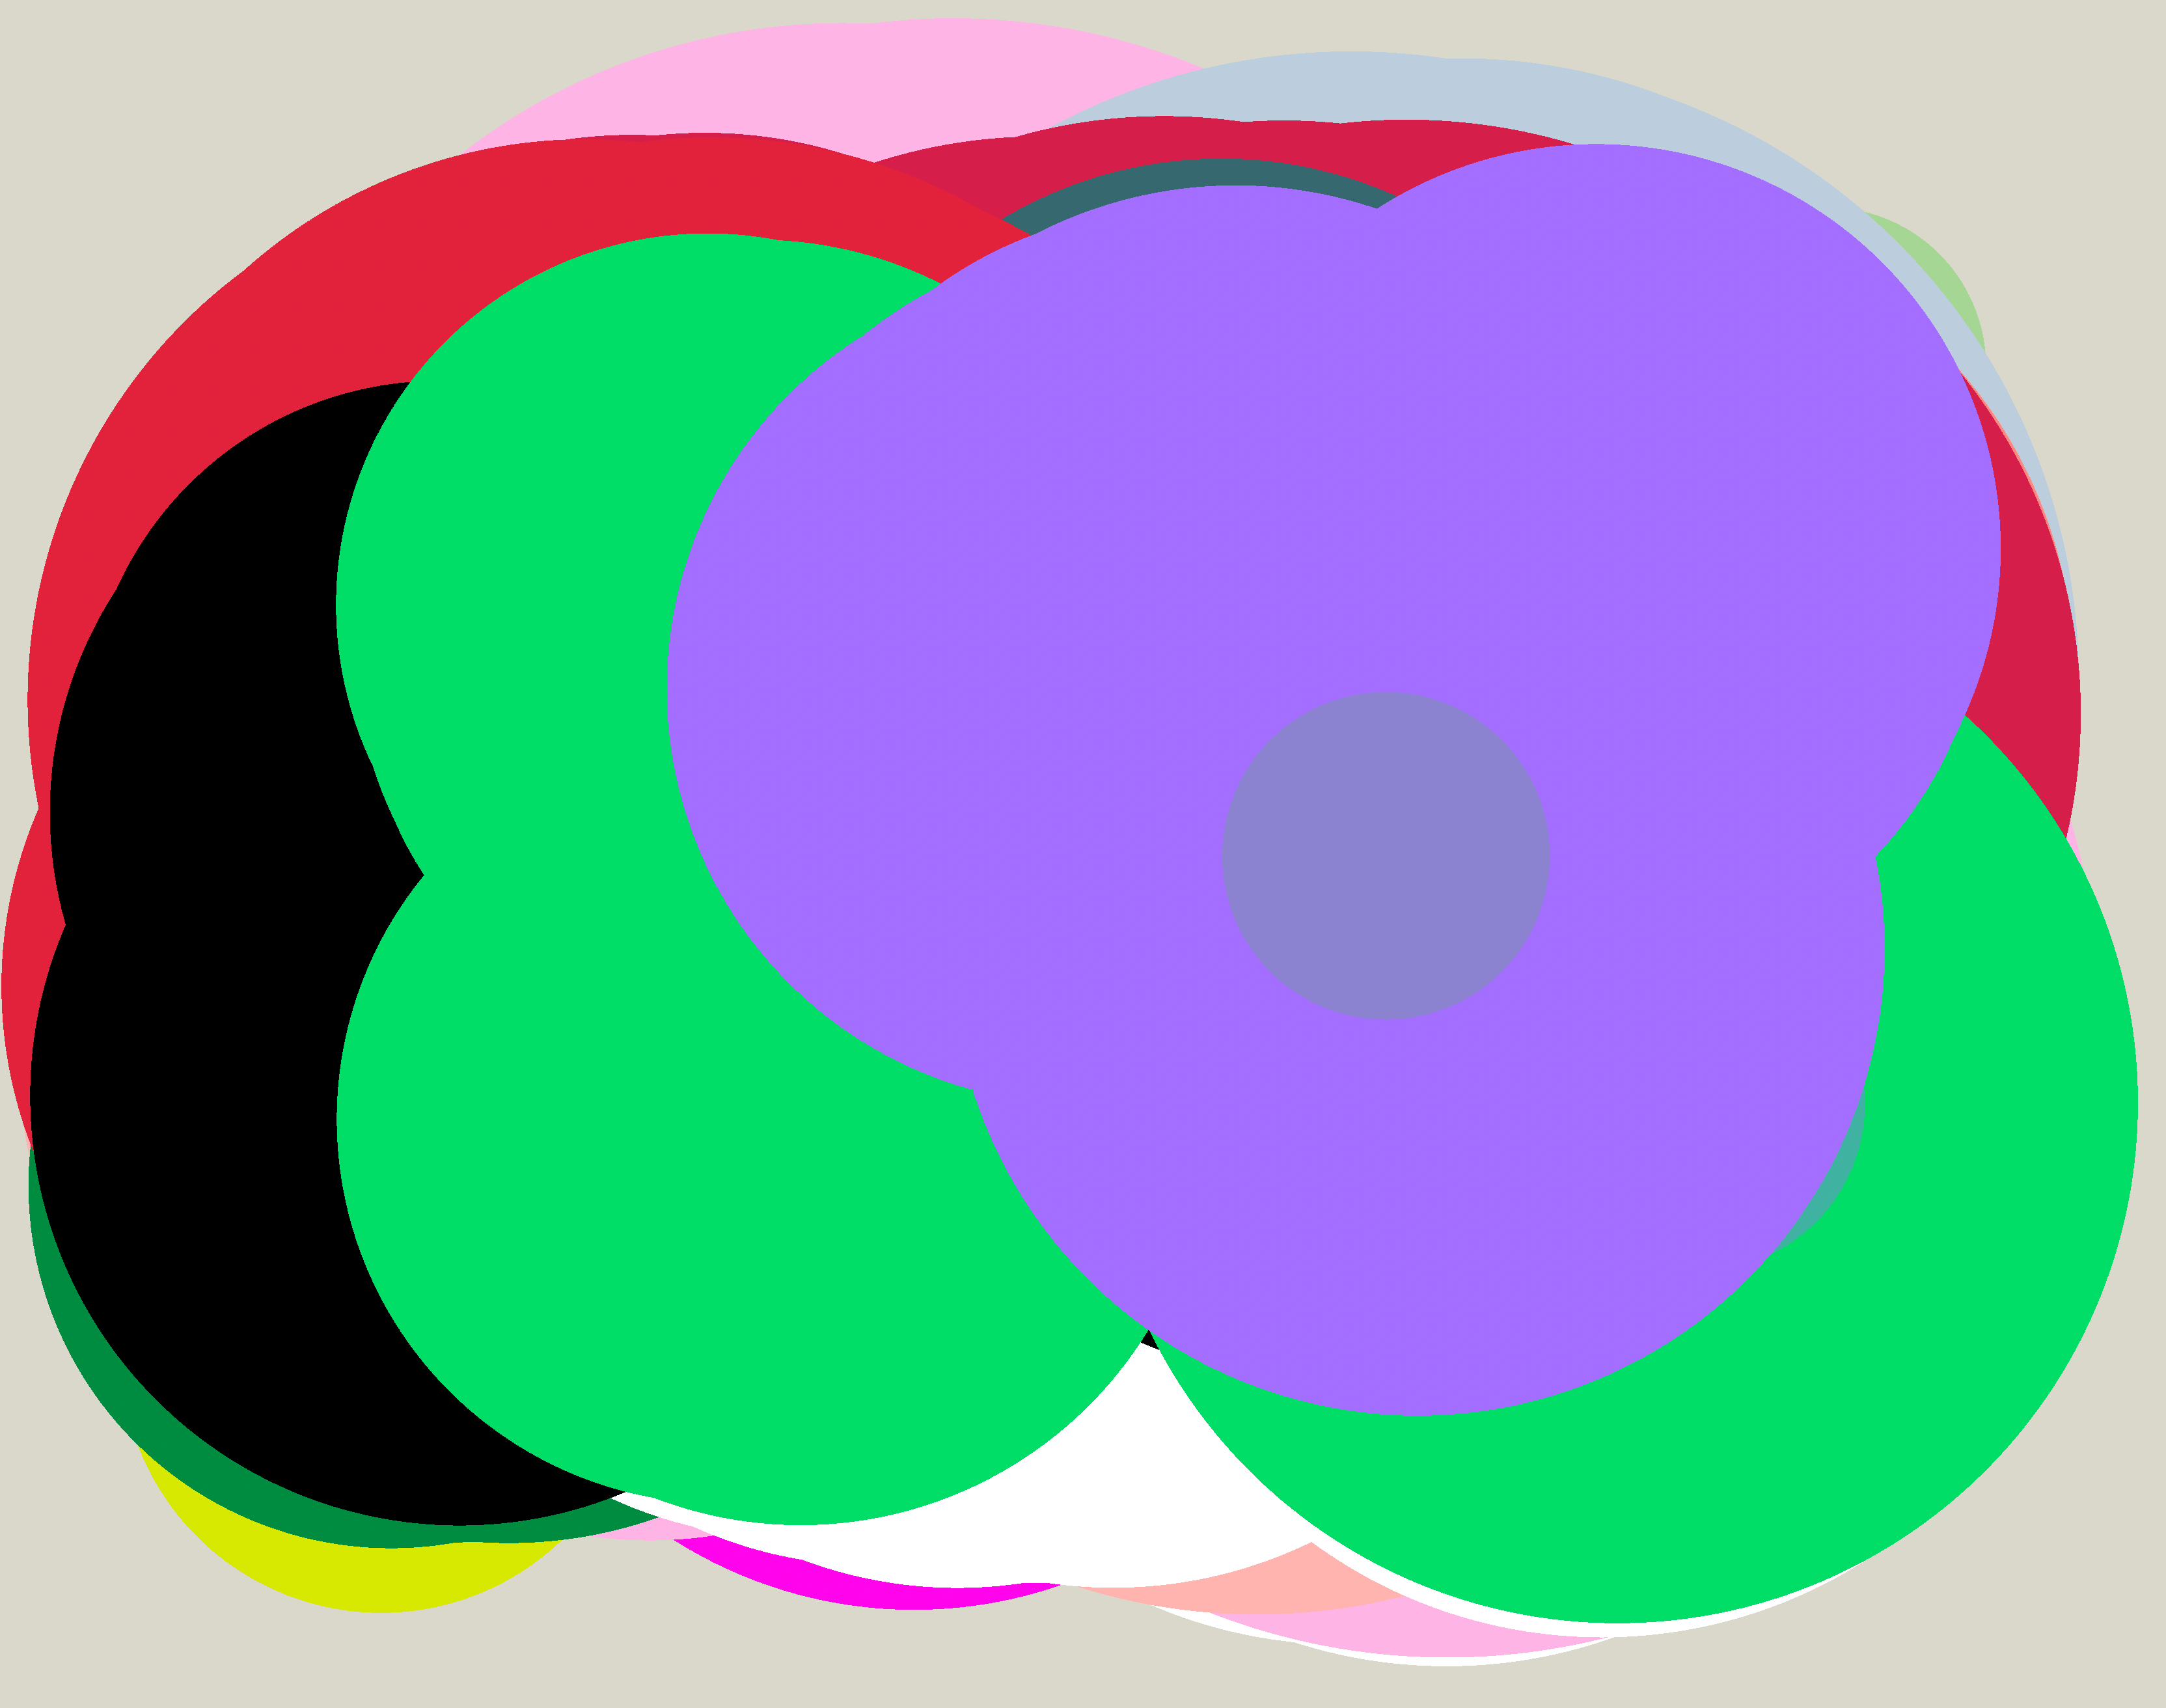
\includegraphics[width=\imwidth]{jack-circles.png}%
  \label{fig:circles}
  \caption{Jack's wonderful circles, without text overlay}
\end{figure}

\begin{figure}
  \centering
  \begin{overpic}[width=\imwidth,unit=1mm,grid,tics=5]{jack-circles.png}
    \put(1, 2){\textbf{(a)}}
    \put(25, 3){\Large\textbf{Jack Bentley}}
  \end{overpic}%
  \hfill
  \begin{tikzpicture}[above right, inner sep=0, outer sep=0]
    \node (image) at (0, 0)
      { 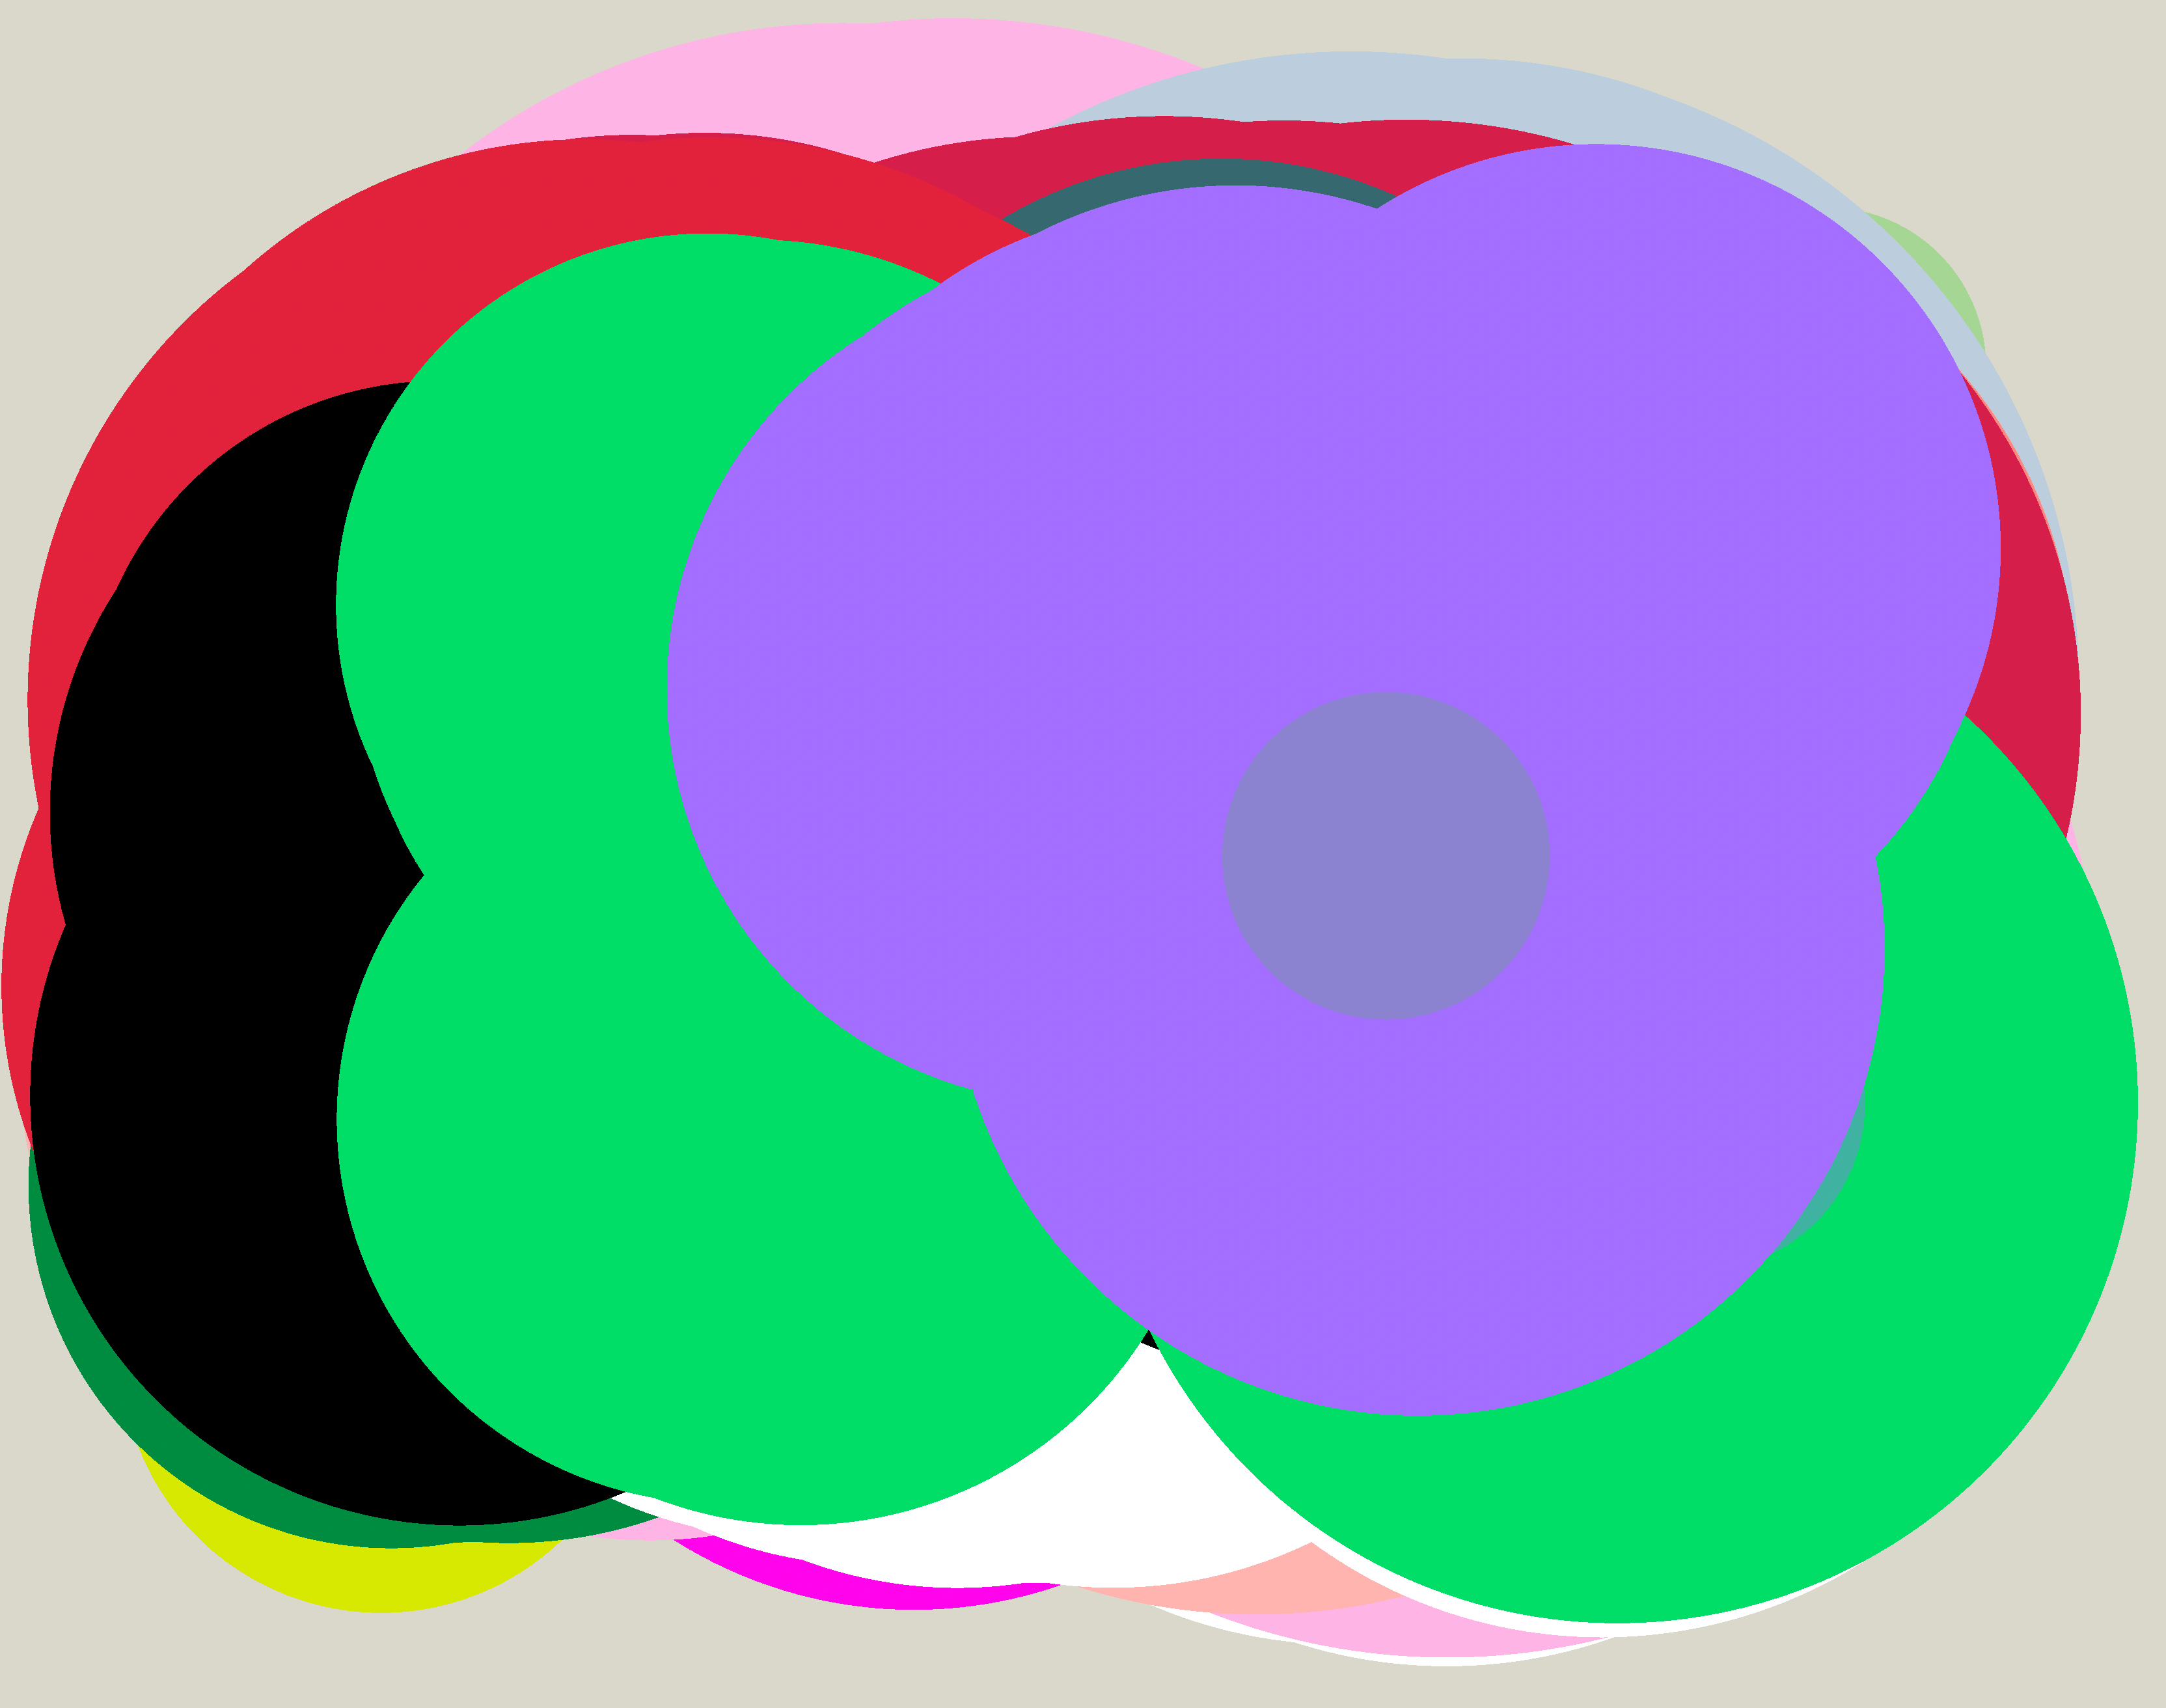
\includegraphics[width=\imwidth]{jack-circles.png} };
    \node (label) at (1mm, 1mm) {\textbf{(b)}};
    \node[above left] (name) at (\imwidth - 1mm, 1mm)
      { \Large \textbf{Jack Bentley} };
    \draw[step=5mm] (image.south west) grid (image.north east);
  \end{tikzpicture}%
  \label{fig:circles}
  \caption{Jack's wonderful circles, with text overlay and a grid}
\end{figure}

\begin{figure}
  \centering
  \begin{overpic}[width=\imwidth,unit=1mm]{jack-circles.png}
    \put(1, 2){\textbf{(a)}}
    \put(25, 3){\Large\textbf{Jack Bentley}}
  \end{overpic}%
  \hfill
  \begin{tikzpicture}[above right, inner sep=0, outer sep=0]
    \node (image) at (0, 0)
      { 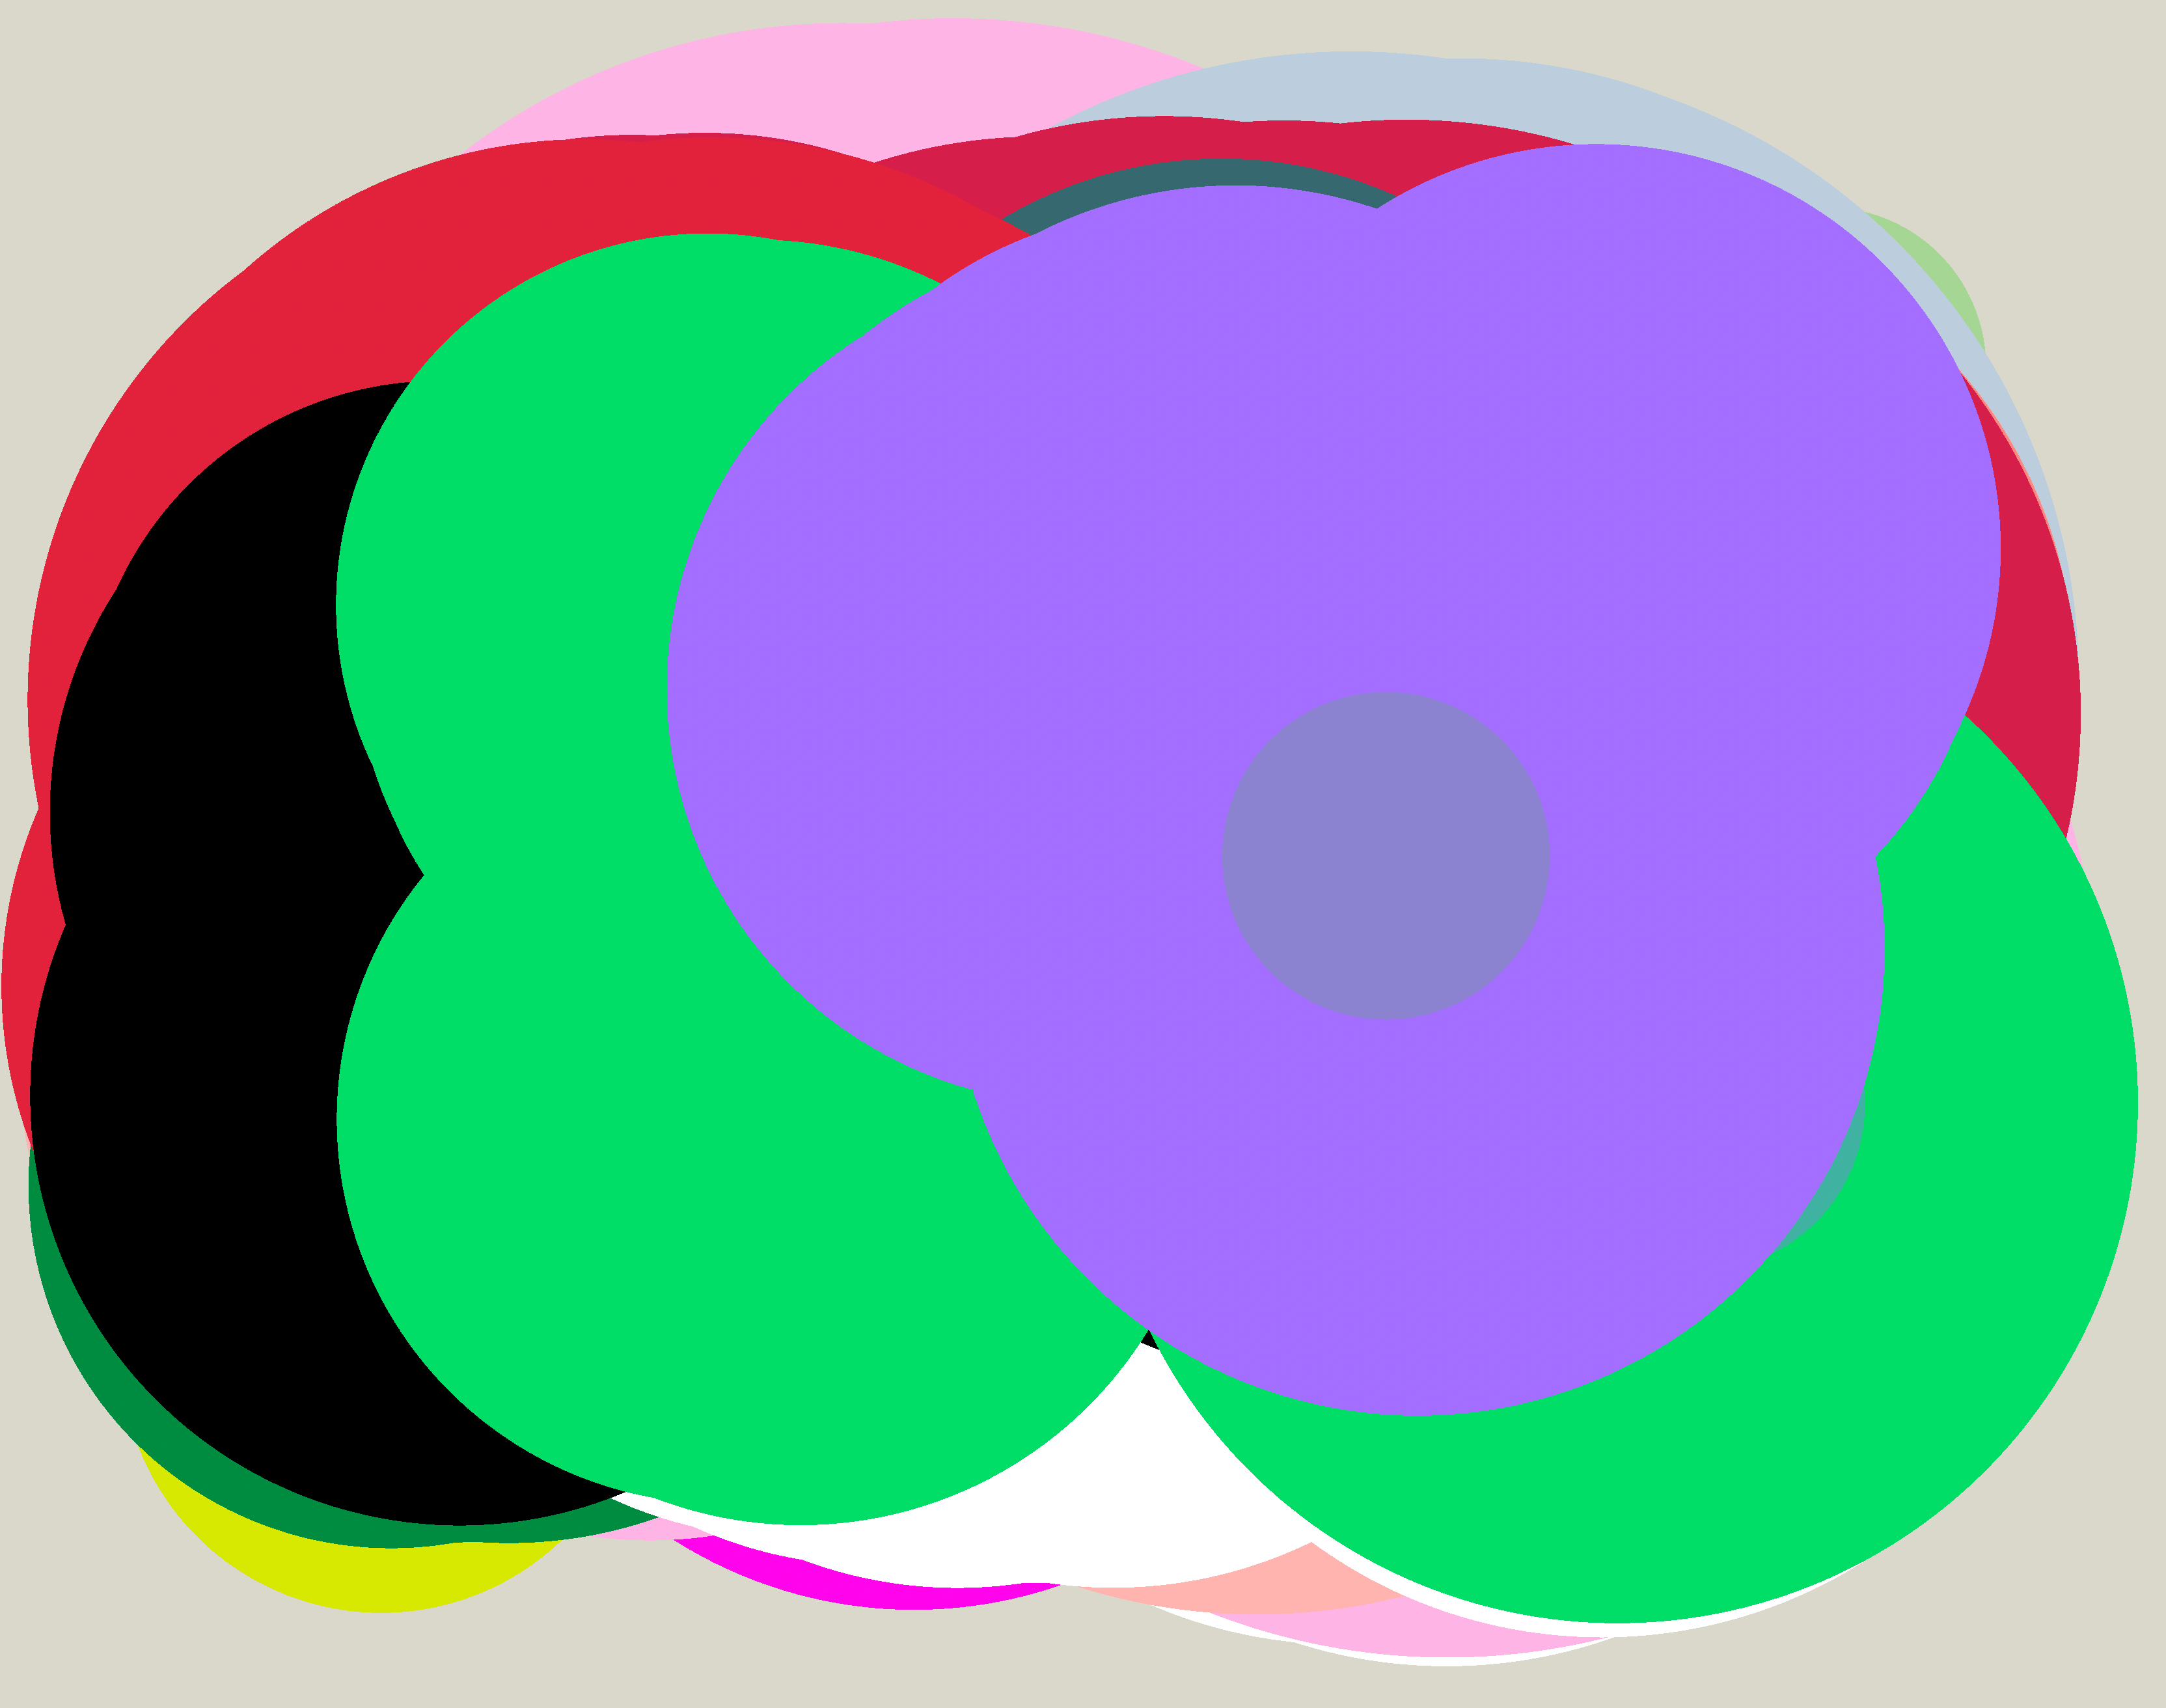
\includegraphics[width=\imwidth]{jack-circles.png} };
    \node (label) at (1mm, 1mm) {\textbf{(b)}};
    \node[above left] (name) at (\imwidth - 1mm, 1mm)
      { \Large \textbf{Jack Bentley} };
  \end{tikzpicture}%
  \label{fig:circles}
  \caption{Jack's wonderful circles, with text overlay and without a grid}
\end{figure}

\begin{figure}
  \centering
  \overlayFigure[width=\imwidth]{\textbf{(a)}}{jack-circles.png}%
  \hfill%
  \annotatedFigure[width=\imwidth]{\textbf{(b)}}{jack-circles.png}%
  \label{fig:circles}
  \caption{Jack's wonderful circles, with text overlay from my newcommand}
\end{figure}

\end{document}
